\begin{wrapfigure}{r}{.5\textwidth} 
    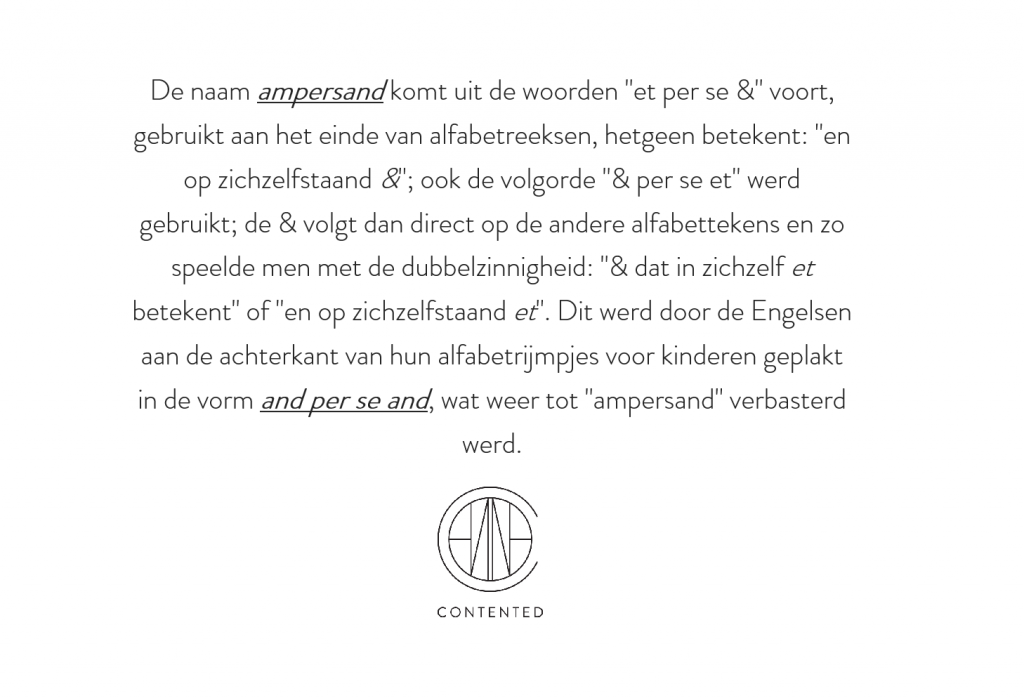
\includegraphics[scale=0.3]
        {Contented_Definitie_Ampersand_Wikipedia-1024x698.png}
    \caption{www.contented.nl/wat-weet-jij-van-het-en-teken-de-ampersand}
    \label{fig:Ampersand definition}
\end{wrapfigure}
The research focuses on the question of the usability of Ampersand, but where does Ampersand (\&) come from.
On the website of www.contend.nl~\footnote{\url{https://www.contented.nl/wat-weet-je-van-het-en-teken-de-ampersand}} we find an explanation for ampersand sign.
When applied to the Ampersand method, the similarity is that both emphasize the meaning "and self-contained".
The Ampersand method is a standalone method that is used.
On the website of Ampersand~\footnote{\url{https://ampersandtarski.gitbook.io/documentation/why-ampersand/business-rules-in-ampersand}} we find an interpretation of the statement "standalone (op zichzelfstaand)".
Ampersand endorses the \acrlong{brm}.
Elements are central here when focusing on primary requirements.
Do not let the process take center stage, but the facts.
In short, Ampersand's self-sufficiency follows the line of \&'s meaning.

During the graduation project, research was conducted into the suitability of Ampersand for designing registers for the government.
These registers are always based on legislation and regulations.
The research focuses on a specific law, namely the \acrshort{big}.

This law does not stand alone.
The associated laws and regulations are the following:
\begin{enumerate}
    \item Wet op de beroepen in de individuele gezondheidszorg
    \item Besluit periodieke registratie Wet BIG
    \item Registratiebesluit BIG
    \item Tuchtrechtbesluit BIG
    \item Regeling periodieke registratie Wet BIG
    \item Regeling tarieven registratie beroepsbeoefenaren Wet BIG
    \item Algemene wet erkenning EU-beroepskwalificaties
\end{enumerate} 
In principle, these laws and regulations are part of an investigation into the suitability of Ampersand.
However, the time that can be spent on the research does not allow to include all parts.
After all, the aim is not to provide a fully elaborated conceptual analysis.
By applying the principle of time-boxing, only a limited part of the legislation and regulations is analyzed and converted to Ampersand scripts.

The results of the study will be discussed in the following chapters.
The research that focuses on the research question "\acrlong{research question}".
By answering the derived questions, we provide a view on the usability of Ampersand.